
\caulc

%%%=============EX_1=============%%%
\begin{ex}%[1D6N3-2]%[TDMT07]%[Bồ Văn Hậu]
	Tập xác định của hàm số $y=\log_2(1-x)$ là
	\choice
	{\True $(-\infty;1)$}
	{$\mathbb{R}\setminus \{1\}$}
	{$(0;1)$}
	{$(1;+\infty)$}
	\loigiai{
		Điều kiện xác định của hàm số $y=\log_2(1-x)$ là $1-x>0$ hay $x<1$.\\
		Vậy tập xác định của hàm số trên là $\mathscr{D}=(-\infty;1)$.
	}
\end{ex}
%%%=============================%%%

%%%=============EX_2=============%%%
\begin{ex}%[1D1H5-3]%[TDMT07]%[Đình Nguyên]
	Nghiệm của phương trình $\tan \left( 2x - \dfrac{\pi}{3} \right) = \sqrt{3}$ là
	\choice
	{$x = \dfrac{\pi}{3} + k\pi$, $k \in \mathbb{Z}$}
	{\True $x = \dfrac{\pi}{3} + \dfrac{k\pi}{2}$, $k \in \mathbb{Z}$}
	{$x = \dfrac{\pi}{6} + \dfrac{k\pi}{2}$, $k \in \mathbb{Z}$}
	{$x = \dfrac{\pi}{3} + \dfrac{k\pi}{2}$, $k \in \mathbb{N}$}
	\loigiai{
		Điều kiện xác định $\cos\left( 2x - \dfrac{\pi}{3}\right)\neq 0
		\Leftrightarrow 2x - \dfrac{\pi}{3} \neq \dfrac{\pi}{2} + k\pi \Leftrightarrow 2x \neq \dfrac{5\pi}{6} + k\pi \Leftrightarrow x \neq \dfrac{5\pi}{12} + \dfrac{k\pi}{2}$\,\,($k \in \mathbb{Z}$).\\
		Ta có \begin{eqnarray*}
			\tan \left( 2x - \dfrac{\pi}{3} \right) = \sqrt{3} &\Leftrightarrow& \tan \left( 2x - \dfrac{\pi}{3} \right) = \tan \dfrac{\pi}{3}\\
			&\Leftrightarrow& 2x - \dfrac{\pi}{3} = \dfrac{\pi}{3} + k\pi\\ 
			&\Leftrightarrow& 2x = \dfrac{2\pi}{3} + k\pi\\
			&\Leftrightarrow& x = \dfrac{\pi}{3} + \dfrac{k\pi}{2},\, k \in \mathbb{Z}\; (\text{thỏa mãn điều kiện}).
		\end{eqnarray*}
	}
\end{ex}
%%%=============================%%%

%%%=============EX_3=============%%%
\begin{ex}%[1D6N3-3]%[TDMT07]%[Trần Văn Thiện]
	Tập giá trị của hàm số $y=3^x$ là
	\choice
	{$\left(-\infty;+\infty\right)$}
	{$\left[0;+\infty\right)$}
	{ $\left(-\infty;0\right)$}
	{\True$\left(0; +\infty\right)$}
	\loigiai{
		Hàm số $y=3^x$ là hàm số mũ có cơ số $a=3>1$ nên luôn đồng biến và liên tục trên $\mathbb{R}$.\\
		Ngoài ra ta có $\lim\limits_{x\to -\infty} y = 0$ và $\lim\limits_{x\to +\infty} y = +\infty$.\\ Do đó tập giá trị của hàm số là $(0; +\infty)$.
	}
\end{ex}
%%%=============================%%%

%%%=============EX_4=============%%%
\begin{ex}%[1D2N2-4]%[TDM-Đề 6]%[Đoàn Văn Mùi]
	Cho cấp số cộng $(u_n)$ có số hạng đầu bằng $1$ và công sai bằng $2$. Số hạng $u_3$ bằng
	\choice
	{$7$}
	{$3$}
	{\True $5$}
	{$4$}
	\loigiai{
		Công thức số hạng tổng quát $u_n = u_1 + (n-1)d$.\\ 
		Suy ra $u_3=u_1+2d=1+2\cdot 2=5$.
	}
\end{ex}
%%%=============================%%%

%%%=============EX_5=============%%%
\begin{ex}%[1H8H7-3]%[TDMT07]%[Nguyễn Trí Minh Tuấn]
	Cho hình chóp $S. ABCD$ có đáy là hình vuông có diện tích bằng $12$, mặt bên $(SAB)$ là tam giác đều và nằm trong mặt phẳng vuông góc với đáy. Thể tích hình chóp $S. ABCD$ bằng
	\choice
	{$6\sqrt{3}$}
	{\True $12$}
	{$36$}
	{$4$}
	\loigiai{
		\immini{
			Do đáy $ABCD$ là hình vuông có diện tích bằng $12$ nên $AB^2 = 12 \Rightarrow AB = 2\sqrt{3}$.\\
			Trong $\triangle ABC$, gọi $H$ là trung điểm của $AB$, khi đó $SH$ là chiều cao của hình chóp và
			\[
			SH = \dfrac{\sqrt{3}}{2}AB = \dfrac{\sqrt{3}}{2}\cdot 2\sqrt{3} = 3.
			\]
			Vậy thể tích hình chóp là
			\[
			V = \dfrac{1}{3}\cdot S_{ABCD}\cdot SH
			= \dfrac{1}{3}\cdot 12 \cdot 3
			= 12.\]
		}{
			\begin{tikzpicture}[line cap=round,line join=round,font=\footnotesize,scale=0.8]
				\coordinate (A) at (0,0);
				\coordinate (B) at (-2,-2);
				\coordinate (D) at (5,0);
				\coordinate (C) at ($(B)+(D)-(A)$);
				\coordinate (H) at ($(A)!.5!(B)$);
				\coordinate (S) at ($(H)+(0,6)$);
				\draw  (S)--(B) (S)--(C) (S)--(D) (B)--(C)--(D);
				\draw[dashed] (S)--(H) (B)--(A)--(D) (S)--(A);
				\foreach \x/\goc in {S/above, A/left, B/left, C/right, D/right, H/below right}
				{
					\draw[fill=black] (\x) circle (1pt) node[\goc] {$\x$};
				}
				\draw ($(H)!0.05!(S)$) -- ($(H)!0.05!(S)+(H)!0.15!(A)-(H)$) -- ($(H)!0.15!(A)$);
			\end{tikzpicture}
	}}
\end{ex}
%%%=============================%%%

%%%=============EX_6=============%%%
\begin{ex}%[VN-MT-4]%[TDM21, Nguyễn Văn Sang]%[2D1N1-2]
	\immini[thm]{
		Cho đồ thị của hàm số $y=f(x)$ như hình vẽ bên. Hỏi hàm số $f(x)$ nghịch biến trên khoảng nào dưới đây?
		\choice[2]
		{$(-5;+\infty)$}
		{\True $(-2;4)$}
		{$(4;+\infty)$}
		{$(-\infty;4)$}
	}{
		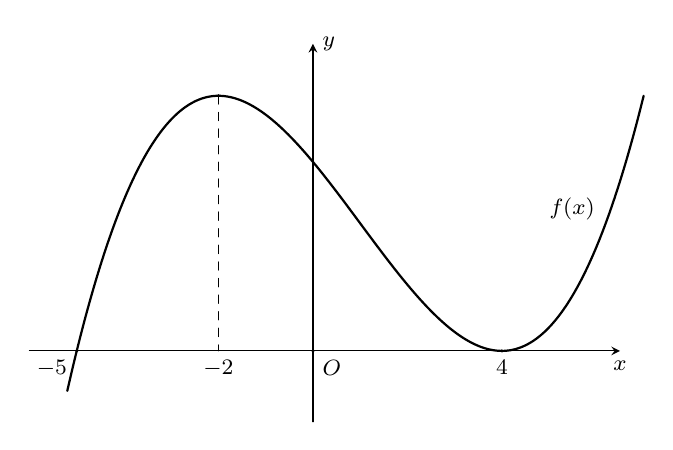
\begin{tikzpicture}[scale=0.6, font=\footnotesize, line join=round, line cap=round, >=stealth]
			\draw[->] (-6,0) -- (6.5,0) node[below] {$x$};
			\draw[->] (0,-1.5) -- (0,6.5) node[right] {$y$};
			\fill (0,0) circle (1pt) node[below right] {$O$};
			\draw[thick, smooth, samples=100, domain=-5.2:7] plot (\x,{0.05*(\x+5)*(\x-4)^2});
			\fill (-2,5.4) circle (1pt);
			\draw[dashed] (-2,5.4) -- (-2,0) node[below] {$-2$};
			\fill (4,0) circle (1pt) node[below] {$4$};
			\fill (-5,0) circle (1pt) node[below left] {$-5$};			
			\node[right] at (4.8,3) {$f(x)$};
		\end{tikzpicture}
	}
	\loigiai{
		Dựa vào đồ thị, ta thấy hàm số nghịch biến (đồ thị đi xuống từ trái sang phải) trên khoảng $(-2;4)$.
	}
\end{ex}
%%%=============================%%%

%%%=============EX_7=============%%%
\begin{ex}%[2D1H2-1]%[TDMT07]%[Phạm Hải Dương]
	Cực tiểu của hàm số $y=x^3-3x$ là
	\choice
	{$(1;-2)$}
	{$(-1;2)$}
	{$x=1$}
	{\True $y = -2$}
	\loigiai{
		Tập xác định $\mathscr{D} = \mathbb{R}$.\\
		Ta có $y'=3x^2-3$; $y''=6x$.\\
		Khi đó $y'=0 \Leftrightarrow 3x^2-3=0 \Leftrightarrow x=\pm 1$.\\
		Bảng biến thiên
		\begin{center}
			\begin{tikzpicture}[font=\normalsize,t style/.style={style=solid}]
				\tkzTabInit[nocadre=false,lgt=1.2,espcl=2.5,deltacl=0.5]%,help]
				{$x$/0.75,$y'$/0.75,$y$/3}
				{$-\infty$,$-1$,$1$,$+\infty$}
				\tkzTabLine{,+,0,-,0,+}
				\path
				($(N13)!0.1!(N12)$) node (A1){$ -\infty $}
				($(N23)!0.7!(N22)$) node (A2){$ 2 $}
				($(N33)!0.2!(N32)$) node (A3){$ -2 $}
				($(N43)!0.8!(N42)$) node (A4){$ +\infty $};
				\foreach \x/\y in {A1/A2,A2/A3,A3/A4}{
					\draw[-stealth] (\x)--(\y);
				}
			\end{tikzpicture}
		\end{center}
		Dựa vào bảng biến thiên và kiểm tra bằng đạo hàm cấp $2$, ta có
		\begin{itemize}
			\item Tại $x=-1$: $y''(-1) = -6 < 0 \Rightarrow$ Hàm số đạt cực đại.
			\item Tại $x=1$: $y''(1) = 6 > 0 \Rightarrow$ Hàm số đạt cực tiểu.
		\end{itemize}
		Giá trị cực tiểu của hàm số là $y(1)=1^3-3 \cdot 1 =-2$.\\
		Vậy cực tiểu của hàm số là $y = -2$.
	}
\end{ex}
%%%=============================%%%

%%%=============EX_8=============%%%
\begin{ex}%[2D1H3-2]%[TDMT07]%[Văn Minh Thoại]
	Giá trị nhỏ nhất của hàm số $f(x)=x^3-6x$ trên $(0;+\infty)$ bằng
	\choice
	{$0$}
	{$4\sqrt{2}$}
	{\True $-4\sqrt{2}$}
	{$-2\sqrt{2}$}
	\loigiai{
		Xét hàm số $f(x)=x^3-6x$ trên $(0;+\infty)$.\\
		Ta có $f'(x)=3x^2-6$.\\
		Khi đó $f'(x)=0 \Leftrightarrow 3x^2-6=0 \Leftrightarrow x^2=2 \Leftrightarrow \hoac{&x=\sqrt{2} \in (0;+\infty)\\&x=-\sqrt{2} \notin (0;+\infty).}$\\
		Bảng biến thiên
		\begin{center}
			
\begin{tikzpicture}
				\tkzTabInit[lgt=1.2,espcl=3]
				{$x$/1,$f'(x)$/1,$f(x)$/2}
				{$0$,$\sqrt{2}$,$+\infty$}
				\tkzTabLine{,-,0,+,}
				\tkzTabVar{+/$0$,-/$-4\sqrt{2}$,+/$+\infty$}
			\end{tikzpicture}
		\end{center}
		Dựa vào bảng biến thiên, giá trị nhỏ nhất của hàm số trên $(0;+\infty)$ là
		$f\left(\sqrt{2}\right) = -4\sqrt{2}$.
	}
\end{ex}
%%%=============================%%%

%%%=============EX_9=============%%%
\begin{ex}%[2D1H2-2]%[TDMT07]%[Lê Phúc]
	\immini[thm]{Cho đồ thị hàm số $y=f'(x)$ như hình vẽ. Hỏi hàm số $f(x)$ có tất cả bao nhiêu điểm cực tiểu?
		\choice
		{$4$}
		{\True $1$}
		{$3$}
		{$2$}}{
		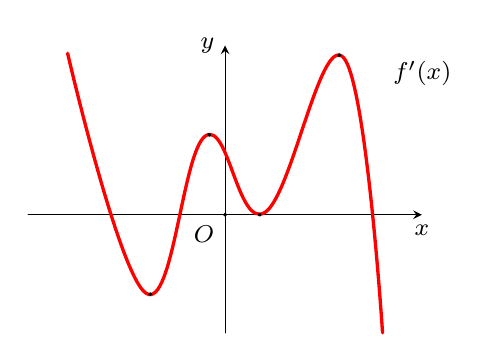
\begin{tikzpicture}[scale=0.5,>=stealth, font=\footnotesize, line join=round, line cap=round]
			\def\xmin{-5} \def\xmax{5}
			\def\ymin{-3} \def\ymax{4.3}
			\tikzset{every node/.style={scale=1.1}}
			%\draw[color=gray!50,dashed] (\xmin,\ymin) grid (\xmax,\ymax);
			\draw[->] (\xmin,0)--(\xmax,0) node [below]{$x$};
			\draw[->] (0,\ymin)--(0,\ymax) node [left]{$y$};
			\node at (0,0) [below left]{$O$};
			\draw[red,very thick] plot[smooth,tension=0.7]coordinates {(-4,4.1) (-2,-2) (-0.5,2) (1,0.05) (3,4) (4,-3)};
			\draw[fill=black]
			(0,0)circle (1 pt);
			\draw[fill=black]
			(-1.9,-2.02)circle (1 pt);
			\draw[fill=black]
			(-0.4,2.03)circle (1 pt);
			\draw[fill=black]
			(0.88,0)circle (1 pt);
			\draw[fill=black]
			(2.9,4.05)circle (1 pt);
			\node at (4,3) [above right]{$f'(x)$};
		\end{tikzpicture}
	}
	\loigiai{
		Gọi hoành độ giao điểm của đồ thị hàm số $y=f'(x)$ và trục $Ox$ lần lượt là $a$, $b$, $c$, $d$ ($a<b<c<d$).\\
		Bảng biến thiên của hàm số $y=f(x)$ là
		\begin{center}
			
\begin{tikzpicture}
				\tkzTabInit[espcl=2.5,lgt=1.5]
				{$x$/0.7,$f'(x)$/0.7,$f(x)$/2.1}
				{$-\infty$,$a$,$b$,$c$,$d$,$+\infty$}
				\tkzTabLine{,+,0,-,0,+,0,+,0,-,}
				\tkzTabVar{-/,+/,-/,R/,+/,-/}
			\end{tikzpicture}
		\end{center}
		Dựa vào bảng biến thiên hàm số $y=f(x)$ ta có hàm số $y=f(x)$ có $1$ điểm cực tiểu.
	}
\end{ex}
%%%=============================%%%

\begin{ex}
%%%=============EX_10=============%%%
\sochc{3}
Cho hình lập phương $ABCD. A'B'C'D'$ có cạnh bằng $6$. 
\begin{chc}%[2H2N1-2]%[TDMT07]%[Vũ Hồng Toàn]
	\immini[thm]{Hỏi tổng $\overrightarrow{AB} + \overrightarrow{AD} + \overrightarrow{AA'}$ bằng vectơ nào dưới đây?
		\choice
		{\True $\overrightarrow{AC'}$}
		{$\overrightarrow{AC}$}
		{$\overrightarrow{A'C}$}
		{$\overrightarrow{A'C'}$}}{
		\begin{tikzpicture}[declare function={a=3; b=0.45*a; h=a;goc=-135;},scale=0.7]
			\path
			(0,0) coordinate (A)
			(a,0) coordinate (D)
			(goc:b) coordinate (B)
			($(B)+(D)-(A)$)coordinate (C)
			\foreach \p in {A,B,C,D} {
				($(\p)+(-90:h)$) coordinate (\p')};
			\draw[dashed] (B')--(A')--(D') (A')--(A);
			\draw (B)--(C)--(C')--(B')--cycle--(A)--(D)--(D')--(C') (C)--(D);
			\foreach \x/\goc in {A/160,B/180,C/0,D/0,A'/160,B'/180,C'/-30,D'/0}{
				\fill (\x) circle (1pt) node[shift={(\goc:7pt)},font=\small]{$\x$};
			}
		\end{tikzpicture}
	}
	\loigiai{
		Áp dụng quy tắc hình hộp cho hình lập phương $ABCD. A'B'C'D'$, ta có
		\[\overrightarrow{AB} + \overrightarrow{AD} + \overrightarrow{AA'}=\overrightarrow{AC'}.\]
	}
\end{chc}
%%%=============================%%%

%%%=============EX_11=============%%%
\begin{chc}%[0H5H4-1]%[TDMT07]%[Huỳnh Trí Thiện]
	\immini[thm]{Góc giữa hai vectơ $\overrightarrow{A'B}$ và $\overrightarrow{CB'}$ bằng
		\choice
		{$60^\circ$}
		{$90^\circ$}
		{\True $120^\circ$}
		{$135^\circ$}}{
		\begin{tikzpicture}[scale=0.5, font=\footnotesize,line join=round, line cap=round, >=stealth]
			\coordinate (A) at (0,0);
			\coordinate (B) at (-2,-2);
			\coordinate (D) at (5,0);
			\coordinate (C) at ($(B)+(D)-(A)$);
			\foreach \i in {A,B,C,D}{\coordinate (\i') at ($(\i)+(0,4)$);}
			\draw (A')--(B')--(C')--(D')--cycle;
			\draw (B)--(B') (C)--(C') (D)--(D') (B)--(C)--(D);
			\draw[dashed,thin](B)--(A)--(A') (A)--(D) ;
			\draw[dashed,->] (A')--(B);
			\draw[->] (C)--(B');
			\foreach \i/\g in {A'/90,B'/90,C'/90,D'/90,A/-90,B/-90,C/-90,D/-90}{\draw[fill=blue](\i) circle (1.5pt) ($(\i)+(\g:5mm)$) node[scale=1]{$\i$};}
		\end{tikzpicture}
	}
	\loigiai{
		Ta có $\overrightarrow{A'B} = \overrightarrow{D'C}$.\\
		Suy ra $\left(\overrightarrow{A'B}, \overrightarrow{CB'}\right) = \left(\overrightarrow{D'C}, \overrightarrow{CB'}\right)=180^{\circ}-\left(\overrightarrow{CD'},\overrightarrow{CB'}\right)=180^{\circ}-\widehat{D'CB'}$.\\
		Xét tam giác $D'CB'$, ta có các cạnh $D'C$, $CB'$, $B'D'$ đều là đường chéo của các mặt hình vuông bằng nhau nên $D'C = CB' = B'D'$.\\
		Suy ra tam giác $D'CB'$ là tam giác đều.\\ Do đó $\widehat{D'CB'} = 60^\circ$.\\
		Suy ra 
		$\left(\overrightarrow{D'C}, \overrightarrow{CB'}\right) = 180^\circ - 60^\circ = 120^\circ$.
	}
\end{chc}
%%%=============================%%%

%%%=============EX_12=============%%%
\begin{chc}%[2H2H1-3]%[TDMT06]%[Nguyễn Sơn Thành]
	Hãy tính $\overrightarrow{AC'} \cdot \overrightarrow{CD}$?
	\choice
	{$0$}
	{$36$}
	{$12\sqrt{3}$}
	{\True $-36$}
	\loigiai{
		\immini{Ta có $\overrightarrow{AC'} = \overrightarrow{AB} + \overrightarrow{AD} + \overrightarrow{AA'}$, $\overrightarrow{CD} = -\overrightarrow{AB}$.\\
			Suy ra
			\begin{eqnarray*}
				&\overrightarrow{AC'} \cdot \overrightarrow{CD} & =\left(\overrightarrow{AB} + \overrightarrow{AD} + \overrightarrow{AA'}\right) \cdot \overrightarrow{CD}\\
				& & =\left(\overrightarrow{AB} + \overrightarrow{AD} + \overrightarrow{AA'}\right) \cdot \left(-\overrightarrow{AB}\right)\\
				& & = -\overrightarrow{AB}^2 - \overrightarrow{AD} \cdot \overrightarrow{AB} - \overrightarrow{AA'} \cdot \overrightarrow{AB}\\
				& & = -6^2 - 0 - 0 = -36.
			\end{eqnarray*}
			$\left( \overrightarrow{AD} \perp \overrightarrow{AB}\Rightarrow \overrightarrow{AD} \cdot \overrightarrow{AB}=0,\,\, \overrightarrow{AA'} \perp \overrightarrow{AB}\Rightarrow \overrightarrow{AA'} \cdot \overrightarrow{AB}=0\right) $
		}{\begin{tikzpicture}[line cap=round, line join=round, font=\footnotesize, >=stealth, scale=0.8]
				\path 
				(0,0) coordinate (A)
				(5,0) coordinate (D)
				(-2,-2) coordinate (B)
				($(D) - (A) + (B)$) coordinate (C)
				($(A) + (0,3)$) coordinate (A')
				($(B) + (0,3)$) coordinate (B')
				($(C) + (0,3)$) coordinate (C')
				($(D) + (0,3)$) coordinate (D')
				;
				\draw[dashed] (A')--(A)--(C') (B)--(A)--(D);
				\draw (A')--(B')--(C')--(D')--cycle (D')--(D)--(C) (B')--(B)--(C)--(C')--cycle;
				\foreach \i/\r in {A/180, B/-135, C/-45, D/0, A'/105, B'/180, C'/-45, D'/45}{
					\filldraw[black] (\i) circle (1pt);
					\draw (\i) circle (1pt);
					\node at ($(\i) + (\r:4mm)$) {$\i$};
				}
		\end{tikzpicture}}
	}
\end{chc}
%%%=============================%%%
\end{ex}


\cauds

%%%=============EX_13=============%%%
\begin{ex}%[2D1H3-1]%[TDMT07]%[Huỳnh Quốc Đạt]
	Cho hàm số $f(x)=\cos {2x}+x$.
	\choiceTF
	{Đạo hàm của hàm số đã cho là $f'(x)=-\sin 2x+1$}
	{\True $f(0)=1$, $f\left(\dfrac{\pi}{4}\right)=\dfrac{\pi}{4}$}
	{Nghiệm của phương trình $f'(x)=0$ trên khoảng $\left(0;\dfrac{\pi}{4}\right)$ là $\dfrac{\pi}{6}$}
	{Giá trị lớn nhất của hàm số $f(x)$ trên đoạn $\left[0;\dfrac{\pi}{4}\right]$ là $\dfrac{\pi+3}{6}$}
	\loigiai{
		\begin{itemchoice}
			\itemch Ta có $f'(x)=-2\sin {2x}+1$.
			\itemch Ta có $f(0)=\cos (2\cdot 0)+0=1$ và $f\left(\dfrac{\pi}{4}\right)=\cos \left(2\cdot \dfrac{\pi}{4}\right)+\dfrac{\pi}{4}=\dfrac{\pi}{4}$.
			\itemch Ta có $f'(x)=0\Leftrightarrow -2\sin {2x}+1=0\Leftrightarrow \sin {2x}=\dfrac{1}{2}\Leftrightarrow \hoac{&2x=\dfrac{\pi}{6}+k2\pi\\&2x=\dfrac{5\pi}{6}+k2\pi}\Leftrightarrow\hoac{&x=\dfrac{\pi}{12}+k\pi\\& x=\dfrac{5\pi}{12}+k\pi.}$\\
			Với $x\in\left(0;\dfrac{\pi}{4}\right) \Leftrightarrow \hoac{&0<\dfrac{\pi}{12}+k\pi<\dfrac{\pi}{4}\\& 0<\dfrac{5\pi}{12}+k\pi<\dfrac{\pi}{4}}\Leftrightarrow \hoac{&-\dfrac{1}{12}<k<\dfrac{1}{6}\\& -\dfrac{5}{12}<k<-\dfrac{1}{6}}\Rightarrow k=0$.\\
			Vậy phương trình có nghiệm duy nhất $x=\dfrac{\pi}{12}$.
			\itemch Ta có $f(0)=1$, $f\left(\dfrac{\pi}{4}\right)=\dfrac{\pi}{4}$, $f\left(\dfrac{\pi}{12}\right)=\dfrac{\sqrt{3}}{2}+\dfrac{\pi}{12}$.\\
			So sánh các giá trị, ta có $f\left(\dfrac{\pi}{12}\right)>f(0)>f\left(\dfrac{\pi}{4}\right)$.\\
			Vậy giá trị lớn nhất của hàm số $f(x)$ trên đoạn $\left[0;\dfrac{\pi}{4}\right]$ bằng $f\left(\dfrac{\pi}{12}\right)=\dfrac{\sqrt{3}}{2}+\dfrac{\pi}{12}$.
		\end{itemchoice}
	}
\end{ex}
%%%=============================%%%

%%%=============EX_14=============%%%
\begin{ex}%[2D1V3-6]%[TDMT07]%[Đỗ Đường Hiếu]
	Công ty X sản xuất một loại sản phẩm hàng hóa với giá bán kì vọng trong ngày là $p(x)=25x+800$ (nghìn đồng) và chi phí mỗi ngày là $C(x)=x^3+600$ (nghìn đồng), trong đó $x\in\mathbb{N}$ là số lượng sản phẩm sản xuất được. Công ty X chỉ sản xuất tối đa $60$ sản phẩm trong $1$ ngày.
	\choiceTF
	{\True Giá bán kì vọng khi công ty bán $20$ sản phẩm là $1{,}3$ triệu đồng}
	{Hàm lợi nhuận của công ty X là $P(x)=-x^3+25x^2+600x-800$ (nghìn đồng)}
	{Để lợi nhuận đạt tối thiểu $12$ triệu đồng mỗi ngày thì công ty sẽ phải sản xuất từ $13$ đến $37$ sản phẩm}
	{\True Sau khi sản xuất được $27$ sản phẩm, càng sản xuất thêm thì lợi nhuận càng giảm}
	\loigiai{
		\begin{itemchoice}
			\itemch Giá bán kì vọng khi công ty bán $20$ sản phẩm là
			\[p(20)=25\cdot 20+800=1300\,(\text{nghìn đồng})=1{,}3\,(\text{triệu đồng}).\]
			\itemch Hàm lợi nhuận của công ty X là
			\[P(x)=p(x)\cdot x-C(x)=(25x+800)x-\left(x^3+600\right)=-x^3+25x^2+800x-600 \,(\text{nghìn đồng}).\]
			\itemch Để lợi nhuận tối thiểu là $12$ triệu đồng, ta có
			\begin{eqnarray*}
				P(x)\ge 12\,000&\Leftrightarrow& -x^3+25x^2+800x-600\ge 12\,000\\
				&\Leftrightarrow& -x^3+25x^2+800x-12\,600\ge 0\\
				&\Leftrightarrow& \hoac{&x\le x_1\approx -25{,}57\\&13{,}18\approx x_2\le x\le x_3\approx 37{,}38.}
			\end{eqnarray*}
			Suy ra, để lợi nhuận đạt tối thiểu $12$ triệu đồng mỗi ngày thì công ty sẽ phải sản xuất từ $14$ đến $37$ sản phẩm.
			\itemch Xét hàm số $P(x)=-x^3+25x^2+800x-600$ với $x\ge 0$.\\
			Ta có $P'(x)=-3x^2+50x+800$, $P'(x)=0\Rightarrow x=\dfrac{80}{3}$.\\
			Bảng biến thiên
			\begin{center}
				
\begin{tikzpicture}
					\tkzTabInit[nocadre=false,lgt=1.2,espcl=2.5,deltacl=0.6]
					{$x$ /1, $y'$ /0.6, $y$ /2}
					{$0$,$\dfrac{80}{3}$,$+\infty$}
					\tkzTabLine{,+,0,-,}
					\tkzTabVar{-/,+/,-/}
				\end{tikzpicture}
			\end{center}
			Ta có $\dfrac{80}{3}\approx 27$.\\ Suy ra, lợi nhuận cao nhất khi sản xuất $27$ sản phẩm.\\ Sau khi sản xuất được $27$ sản phẩm, càng sản xuất thêm thì lợi nhuận càng giảm.
		\end{itemchoice}
	}
\end{ex}
%%%=============================%%%

%%%=============EX_15=============%%%
\begin{ex}%[2H2V1-3]%[TDMT07]%[Dương Công Tạo]
	\immini[thm]{Cho một mô hình đồ chơi có dạng hình lăng trụ đứng tam giác $ABC. A'B'C'$. Biết rằng $AB=8$, $AC=10$, $\widehat{BAC}=60^{\circ}$, $AA'=12$. Đặt $\overrightarrow{AB}=\overrightarrow{b}$, $\overrightarrow{AC}=\overrightarrow{c}$, $\overrightarrow{AA'}=\overrightarrow{a}$. Gọi $M$ và $N$ lần lượt là trung điểm của các cạnh $AB$ và $B'C'$.
		\choiceTF
		{\True $\overrightarrow{a}^2=144$, $\overrightarrow{b}^2=64$, $\overrightarrow{c}^2=100$}
		{$\overrightarrow{a} \cdot \overrightarrow{b}=0$, $\overrightarrow{b} \cdot \overrightarrow{c}=50$, $\overrightarrow{c} \cdot \overrightarrow{a}=0$}
		{\True $\overrightarrow{AM}=\dfrac{1}{2} \overrightarrow{b}$; $\overrightarrow{A'N}=\dfrac{1}{2} (\overrightarrow{b}+\overrightarrow{c})$}
		{$MN=2\sqrt{37}$}}
	{\begin{tikzpicture}
			\def\a{3}
			\def\h{3.5}
			\path 	(0:0) coordinate (A)
			++(0:\a) coordinate (C)
			++(-150:3*\a/4) coordinate (B)
			($(A)+(90:\h)$) coordinate (A')
			($(B)+(90:\h)$) coordinate (B')
			($(C)+(90:\h)$) coordinate (C')
			($(A)!.5!(B)$) coordinate (M)
			($(C')!.5!(B')$) coordinate (N);
			\draw[dashed] 	(A)--(C)	(M)--(N);
			\draw	(C)--(C') 	(B)--(B')	(A)--(A') (A)--(B)--(C) (A')--(B')--(C')--cycle;
			\foreach \x/\g in {A/180,B/-45,C/0,A'/180,B'/-45,C'/0,M/-135,N/135}
			\fill[black] 	(\x) circle (1pt)
			($(\g:3.5mm)+(\x)$) node {$\x$};	
		\end{tikzpicture}
	}
	\loigiai{
		\begin{itemchoice}
			\itemch Ta có $\overrightarrow{a}^2=12^2=144$, $\overrightarrow{b}^2=8^2=64$ và $\overrightarrow{c}^2=10^2=100$.
			\itemch Ta có
			\begin{itemize}
				\item Vì đây là khối lăng trụ đứng nên $AA'\perp AB$ hay $\overrightarrow{a}\perp \overrightarrow{b}$. Suy ra $\overrightarrow{a} \cdot \overrightarrow{b}=0$;
				\item $\overrightarrow{b} \cdot \overrightarrow{c}=\left|\overrightarrow{b}\right| \cdot \left|\overrightarrow{c}\right|\cdot\cos60^\circ=8 \cdot 10\cdot\cos60^\circ=40$;
				\item Vì đây là khối lăng trụ đứng nên $AA'\perp AC$ hay $\overrightarrow{c}\perp \overrightarrow{a}$. Suy ra $\overrightarrow{c} \cdot \overrightarrow{a}=0$.
			\end{itemize}
			\itemch Ta có
			\begin{itemize}
				\item $M$ là trung điểm cạnh $AB$ nên $\overrightarrow{AM}=\dfrac{1}{2}\overrightarrow{AB}=\dfrac{1}{2}\overrightarrow{b}$.
				\item $N$ là trung điểm cạnh $B'C'$ nên $\overrightarrow{A'N}=\dfrac{1}{2}\left(\overrightarrow{A'B'}+\overrightarrow{A'C'}\right)=\dfrac{1}{2}\left(\overrightarrow{b}+\overrightarrow{c}\right)$.
			\end{itemize}
			\itemch Ta có
			$\overrightarrow{AN}=\overrightarrow{AA'}+\overrightarrow{A'N}=\overrightarrow{a}+\dfrac{1}{2}\left(\overrightarrow{b}+\overrightarrow{c}\right)=\dfrac{1}{2}\left(2\cdot\overrightarrow{a}+\overrightarrow{b}+\overrightarrow{c}\right)$.
			\allowdisplaybreaks
			\begin{eqnarray*}
				\overrightarrow{MN}&=&\overrightarrow{AN}-\overrightarrow{AM}\\
				&=&\dfrac{1}{2}\left(2\cdot\overrightarrow{a}+\overrightarrow{b}+\overrightarrow{c}\right)-\dfrac{1}{2}\overrightarrow{b}\\
				&=&\dfrac{1}{2}\left(2\cdot\overrightarrow{a}+\overrightarrow{c}\right).
			\end{eqnarray*}
			Khi đó \allowdisplaybreaks
			\begin{eqnarray*}
				MN=\left|\overrightarrow{MN}\right|&=&\dfrac{1}{2}\sqrt{\left(\left|2\cdot\overrightarrow{a}-\overrightarrow{c}\right|\right)^2}\\
				&=&\dfrac{1}{2}\sqrt{4\cdot\left|\overrightarrow{a}\right|^2+\left|\overrightarrow{c}\right|^2-4\cdot\overrightarrow{a}\cdot\overrightarrow{c}}\\
				&=&\dfrac{1}{2}\sqrt{4\cdot 12^2+10^2-4\cdot 0}\\
				&=&13.
			\end{eqnarray*}
		\end{itemchoice}
	}
\end{ex}
%%%=============================%%%

%%%=============EX_16=============%%%
\begin{ex}%[2D1V5-7]%[TDMT07]%[Nguyễn Tấn Linh]
	Cho hàm số $f(x)=\dfrac{x^2-2x+1}{x+2}$ có đồ thị $(C)$.
	\choiceTF
	{\True $(C)$ có tiệm cận đứng là $x=-2$ và tiệm cận xiên là $y=x-4$}
	{\True $(C)$ có tâm đối xứng là $I(-2;-6)$}
	{Có tất cả $6$ điểm có toạ độ nguyên dương nằm trên $(C)$}
	{\True Có tất cả $20$ tam giác có các đỉnh có toạ độ nguyên nằm trên $(C)$}
	\loigiai
	{
		Ta có $y=\dfrac{x^2-2x+1}{x+2} = x-4 + \dfrac{9}{x+2}$.
		\begin{itemchoice}
			\itemch Ta có $\lim\limits_{x \to -2^+} y = +\infty$ nên $x=-2$ là tiệm cận đứng.\\
			$\lim\limits_{x \to \pm \infty} [y-(x-4)] = \lim\limits_{x \to \pm \infty} \dfrac{9}{x+2} = 0$ nên $y=x-4$ là tiệm cận xiên.
			\itemch Tọa độ tâm đối xứng $I$ là nghiệm của hệ phương trình tạo bởi hai đường tiệm cận
			\begin{eqnarray*}
				\heva{&x=-2\\&y=x-4} \Leftrightarrow \heva{&x=-2\\&y=-6.}
			\end{eqnarray*}
			Vậy $I(-2;-6)$.
			\itemch Điểm $M(x;y) \in (C)$ có tọa độ nguyên khi và chỉ khi
			$
			\heva{&x \in \mathbb{Z} \setminus \{-2\}\\ &x+2 \in \text{Ư}(9)=\{\pm 1; \pm 3; \pm 9\}.}
			$\\
			Ta có bảng các điểm có tọa độ nguyên
			\begin{center}
				\begin{tabular}{|c|c|c|c|c|c|c|}
					\hline
					$x+2$ & $-9$ & $-3$ & $-1$ & $1$ & $3$ & $9$ \\
					\hline
					$x$ & $-11$ & $-5$ & $-3$ & $-1$ & $1$ & $7$ \\
					\hline
					$y$ & $-16$ & $-12$ & $-16$ & $4$ & $0$ & $4$ \\
					\hline
				\end{tabular}
			\end{center}
			Các điểm có tọa độ nguyên dương (hoành độ và tung độ đều dương) là $(7;4)$.\\ Vậy chỉ có $1$ điểm thỏa mãn.
			\itemch Từ bảng trên, ta thấy có $6$ điểm có tọa độ nguyên thuộc đồ thị $(C)$.\\
			Vì $(C)$ là đồ thị hàm phân thức bậc hai trên bậc nhất (dạng hypebol) nên một đường thẳng bất kỳ cắt $(C)$ tại tối đa $2$ điểm.\\ Do đó, không có $3$ điểm nào trong $6$ điểm trên thẳng hàng.\\
			Số tam giác tạo thành là $\mathrm{C}_6^3 = 20$.
		\end{itemchoice}
	}
\end{ex}
%%%=============================%%%


\caukq

%%%=============EX_17=============%%%
\begin{ex}%[2D1V3-6]%[TDMT07]%[Lương Pho]
	\immini[thm]{Một trang sách có dạng hình chữ nhật với diện tích là $384$ cm$^2$. Sau khi để lề trên và lề dưới đều là $3$ cm, để lề trái và lề phải đều là $4$ cm. Phần còn lại của trang sách được in chữ. Hãy tính diện tích lớn nhất của phần in chữ trên trang sách theo centimet vuông (\textit{làm tròn kết quả đến hàng đơn vị}).
	}{
		\begin{tikzpicture}[font=\footnotesize, scale=1, line join =round, line cap= round, >= stealth,
			declare function={a=0.8;b=0.6;d=5;r=4;}]
			\draw (0,0) rectangle (r,d);
			\draw[fill=yellow!40] (a,b) rectangle (r-a,d-b);
			\draw[<->] (r/2,0)--(r/2,b) node[pos=0.5,right] {$3$};
			\draw[<->] (r/2,d-b)--(r/2,d) node[pos=0.5,right] {$3$};
			\draw[<->] (0,d/2)--(a,d/2) node[pos=0.5,above] {$4$};
			\draw[<->] (r,d/2)--(r-a,d/2) node[pos=0.5,above] {$4$};
			\path (r/2,d-b)--(r/2,b) node[pos=0.5, sloped,above]{Phần in chữ};
		\end{tikzpicture}
	}
	\par\shortans[0]{160}
	\loigiai{
		Gọi $x$, $y$ (cm) lần lượt là chiều rộng và chiều dài của trang sách ($x$, $y > 0$).\\
		Theo đề bài, ta có diện tích trang sách là
		\[xy = 384 \Rightarrow y = \dfrac{384}{x}.\]
		Điều kiện để có phần in chữ là: $x > 4 + 4 = 8$ và $y > 3 + 3 = 6$.\\
		Khi đó, phần in chữ là một hình chữ nhật có
		\begin{itemize}
			\item Chiều rộng $x - 8$ (cm).
			\item Chiều dài $y - 6$ (cm).
		\end{itemize}
		Diện tích phần in chữ là
		$S = (x - 8)(y - 6) = (x - 8)\left(\dfrac{384}{x} - 6\right)=432 - 6x- \dfrac{3\,072}{x}$.\\
		Xét hàm số $f(x) = 432 - 6x - \dfrac{3\,072}{x}$ với $x > 8$.\\
		Ta có $f'(x) = -6 + \dfrac{3\,072}{x^2}= 0 \Leftrightarrow x^2 = 512 \Leftrightarrow x = 16\sqrt{2}$, (do $x>8$).\\
		Bảng biến thiên
		\begin{center}
			
\begin{tikzpicture}
				\tkzTabInit[nocadre=false,lgt=1.2,espcl=3,deltacl=0.5]
				{$x$/0.7,$f'(x)$/0.7, $f(x)$/2}
				{$8$, $16\sqrt{2}$, $+\infty$}
				\tkzTabLine{,+, 0,- ,} 
				\tkzTabVar{-/$0$, +/$f\left(16\sqrt{2}\right)$, -/$-\infty$}
			\end{tikzpicture}
		\end{center}
		Ta thấy hàm $f(x)$ đạt giá trị lớn nhất $\max\limits_{(8;+\infty)} f(x)=432 - 192\sqrt{2}$ tại $x = 16\sqrt{2}$.\\
		Vậy diện tích lớn nhất của phần in chữ trên trang sách là $432 - 192\sqrt{2} \approx 160\,\left(\text{cm}^2\right)$.
	}
\end{ex}
%%%=============================%%%

%%%=============EX_18=============%%%
\begin{ex}%[1H8V5-4]%[TDMT07]%[Hà Văn Hảo]
	Cho hình lăng trụ $ABCD. A'B'C'D'$ có thể tích bằng $288$ và có đáy là hình vuông cạnh bằng $6$. Biết hình chiếu vuông góc của $A$ trên mặt phẳng $(A'B'C'D')$ là trọng tâm của $\triangle A'B'C'$. Hãy tính khoảng cách giữa hai đường thẳng $AA'$ và $B'C'$ (\textit{làm tròn kết quả đến hàng phần mười}).
	\par
	\shortans[0]{5,4}
	\loigiai{
		Diện tích đáy hình vuông $A'B'C'D'$ là $S = 6^2 = 36$.\\
		Chiều cao của khối lăng trụ là $h = \dfrac{V}{S} = \dfrac{288}{36} = 8$.\\
		Gọi $H$ là hình chiếu của $A$ lên $(A'B'C'D')$ và $O$ là tâm của hình vuông $A'B'C'D'$.\\
		Ta có $AH = 8$, $AC=BD=6\sqrt{2}$ và $H$ là trọng tâm $\triangle A'B'C'$.
		\immini{Chọn hệ trục tọa độ $Oxyz$ như hình vẽ, với $O\left(0;0;0\right)$, $A'\left(0;-3\sqrt{2};0\right)$, $B'\left(-3\sqrt{2};0;0\right)$, $C'\left(0;3\sqrt{2};0\right)$.\\
			Khi đó tọa độ trọng tâm $H$ của $\triangle A'B'C'$ là $H\left(-\sqrt{2};0;0\right)$.\\
			Vì $AH \perp (A'B'C'D')$ và $AH=8$ nên $A(-\sqrt{2}; 0; 8)$.\\
			Ta xác định các vectơ chỉ phương:
			\begin{itemize}
				\item $\overrightarrow{A'A} = \left(-\sqrt{2};3\sqrt{2};8\right)$.
				\item $\overrightarrow{B'C'} = \left(3\sqrt{2};3\sqrt{2};0\right)$.
				\item $\overrightarrow{A'B'} = \left(-3\sqrt{2};3\sqrt{2};0\right)$.
			\end{itemize}
		}{
			\begin{tikzpicture}[scale=1,>=stealth, font=\footnotesize, line join=round, line cap=round,declare function={a=3; b=0.5*a; h=0.9*a;}]
				\path (0:0) coordinate (A)
				(210:b) coordinate (D)
				($(D)+(a,0)$) coordinate (C)
				(a,0) coordinate (B)
				($(B)!1/3!(D)$) coordinate (H)
				(intersection of B--D and A--C) coordinate (O)
				\foreach \x in {A,B,C,D}{(\x)++(50:h) coordinate (\x1)}
				($(A1)+(O)-(H)$) coordinate (O1)
				(intersection of A1--D1 and O--O1) coordinate (I);
				\draw[dashed] (A1)--(A)--(C) (D)--(B)--(A)--cycle (H)--(A1) (O)--(I);
				\draw (D)--(D1)--(A1)--(B1)--(B)--(C)--cycle (D1)--(C1)--(B1) (C1)--(C);
				\draw[-stealth] (D)--($(O)!1.3!(D)$)node[above]{$x$};
				\draw[-stealth] (C)--($(O)!1.7!(C)$)node[above]{$y$};
				\draw[-stealth] (I)--($(O)!1.4!(I)$)node[left]{$z$};
				\draw pic[draw,angle radius=1.2mm]{right angle=A1--H--B};
				\draw pic[draw,angle radius=1.2mm]{right angle=I--O--B};
				\foreach \x/\goc/\t in {A/150/A',B/-30/B',C/-120/C',H/-60/H,O/-90/O,D/-90/D',A1/90/A,B1/90/B,C1/90/C,D1/90/D}
				\fill (\x) circle (1pt) node[shift={(\goc:7pt)},font=\scriptsize]{$\t$};
			\end{tikzpicture}
		}
		\noindent
		Tích có hướng của hai vectơ chỉ phương:
		\[ \left[\overrightarrow{A'A}, \overrightarrow{B'C'} \right] = \left(
		\begin{vmatrix} 3\sqrt{2} & 8 \\ 3\sqrt{2} & 0 \end{vmatrix};
		\begin{vmatrix} 8 & -\sqrt{2} \\ 0 & 3\sqrt{2} \end{vmatrix};
		\begin{vmatrix} -\sqrt{2} & 3\sqrt{2} \\ 3\sqrt{2} & 3\sqrt{2} \end{vmatrix} \right)
		= \left(-24\sqrt{2};24\sqrt{2};-24\right).\]
		Khoảng cách giữa hai đường thẳng chéo nhau $AA'$ và $B'C'$ là
		\[\mathrm{d}\left(AA', B'C'\right) = \dfrac{\left| \left[ \overrightarrow{A'A}, \overrightarrow{B'C'} \right] \cdot \overrightarrow{A'B'} \right|}{\left| \left[\overrightarrow{A'A}, \overrightarrow{B'C'} \right] \right|} = \dfrac{288}{\sqrt{2\,880}} = \dfrac{288}{24\sqrt{5}} = \dfrac{12}{\sqrt{5}} \approx 5{,}4.\]
		Vậy khoảng cách giữa hai đường thẳng $AA'$ và $B'C'$ bằng $5{,}4$.
	}
\end{ex}
%%%=============================%%%

%%%=============EX_19=============%%%
\begin{ex}%[1D2V3-8]%[TDMT07]%[Võ Hiệp]
	\immini[thm]{	Từ độ cao $58$ m của tháp nghiêng Pisa nước Ý, người ta thả một quả bóng cao su chạm xuống đất. Giả sử mỗi lần chạm đất quả bóng bị mất năng lượng và chỉ nảy lên độ cao cực đại bằng $0{,}3$ lần độ cao cực đại mà quả bóng đạt được ở lần nảy lên ngay trước đó. Tính tổng quãng đường mà quả bóng đi được tính từ lúc bắt đầu thả cho tới khi quả bóng nằm yên trên mặt đất ({\it tính theo đơn vị mét và làm tròn kết quả đến hàng đơn vị}).
	}{
		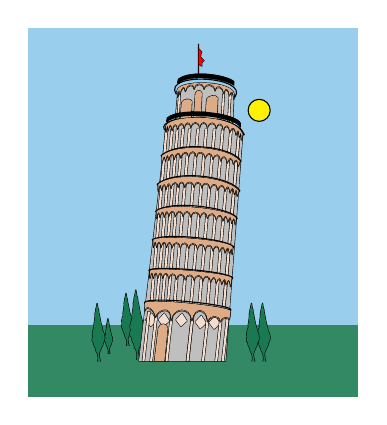
\begin{tikzpicture}[line join=round, line cap=round,scale=1,transform shape,scale=.7]
			\clip (-3,-3.5) rectangle (3,3.2);
			\definecolor{lightcornflowerblue}{rgb}{0.6, 0.81, 0.93}
			\definecolor{cadmiumgreen}{rgb}{0.0, 0.42, 0.24}
			\definecolor{trueblue}{rgb}{0.0, 0.45, 0.81}
			\definecolor{tumbleweed}{rgb}{0.87, 0.67, 0.53}%màu cát
			\tikzset{thap/.pic={%Xây từ dưới lên
					\def\T{
						(-.88,-1.78)%1
						..controls +(40:.17) and +(120:.1) ..  (.686,-1.91)--(.68,-1.94)
						..controls +(120:.1) and +(40:.12) ..  (-.87,-1.81)
						--cycle
						(-.8,-1.2)%2
						..controls +(40:.14) and +(120:.14) ..  (.72,-1.34)--(.7,-1.36)
						..controls +(120:.1) and +(40:.12) ..  (-.78,-1.23)
						--cycle
						(-.74,-.65)%3
						..controls +(40:.22) and +(120:.17) ..  (.74,-.78)--(.72,-.8)
						..controls +(120:.15) and +(40:.15) ..  (-.72,-.67)
						--cycle
						(-.68,-.13)%4
						..controls +(40:.34) and +(110:.2) ..  (.8,-.26)--(.78,-.28)
						..controls +(110:.17) and +(40:.27) ..  (-.66,-.15)
						--cycle
						(-.65,.36)%5
						..controls +(40:.44) and +(120:.3) ..  (.85,.24)--(.83,.22)
						..controls +(130:.35) and +(40:.35) ..  (-.63,.34)
						--cycle
						(-.58,.88)%6
						..controls +(40:.44) and +(120:.3) ..  (.87,.78)--(.85,.76)
						..controls +(130:.35) and +(40:.35) ..  (-.56,.86)
						--cycle
						(-.52,1.35)%7
						..controls +(120:.32) and +(110:.47) ..  (.93,1.26)--(.9,1.25)
						..controls +(110:.43) and +(110:.27) ..  (-.49,1.35)
						--cycle
						(-.31,2)%8
						..controls +(120:.47) and +(55:.46) ..  (.76,1.94)--(.74,1.94)
						..controls +(75:.31) and +(115:.28) ..  (-.28,2)
						--cycle
						(-.48,1.5)
						..controls +(40:.33) and +(110:.2) ..  (.86,1.4)
						(-.476,1.52)
						..controls +(40:.33) and +(110:.2) ..  (.86,1.42)
						(-.472,1.54)
						..controls +(40:.33) and +(110:.2) ..  (.86,1.44)
						(-.468,1.56)
						..controls +(40:.33) and +(110:.2) ..  (.86,1.46)
						(-.28,2.2)
						..controls +(40:.27) and +(140:.2) ..  (.74,2.16)
						(-.276,2.22)
						..controls +(40:.27) and +(140:.2) ..  (.74,2.18)
						(-.272,2.24)
						..controls +(40:.27) and +(140:.2) ..  (.74,2.2)
						(-.268,2.26)
						..controls +(40:.27) and +(140:.2) ..  (.74,2.22)
						;}
					\draw \T;
					%\fill[tumbleweed] \T;
			}}
			\tikzset{rao/.pic={%Rào
					\def\R{
						(-.48,1.5)
						..controls +(40:.33) and +(110:.2) ..  (.86,1.4)
						(-.476,1.52)
						..controls +(40:.33) and +(110:.2) ..  (.86,1.42)
						(-.472,1.54)
						..controls +(40:.33) and +(110:.2) ..  (.86,1.44)
						(-.468,1.56)
						..controls +(40:.33) and +(110:.2) ..  (.86,1.46)
						(-.28,2.2)
						..controls +(40:.27) and +(140:.2) ..  (.74,2.16)
						(-.276,2.22)
						..controls +(40:.27) and +(140:.2) ..  (.74,2.18)
						(-.272,2.24)
						..controls +(40:.27) and +(140:.2) ..  (.74,2.2)
						(-.268,2.26)
						..controls +(40:.27) and +(140:.2) ..  (.74,2.22)
						;}
					\draw \R;
					%\fill[tumbleweed] \R;
			}}
			\tikzset{co/.pic={%Cờ
					\def\C{
						(0.1,2.3)--(.1,2.9)
						(.1,2.82)
						..controls +(-40:.2) and +(140:.22) ..  (.2,2.6)
						..controls +(-60:0) and +(100:.1) ..(.16,2.5)
						..controls +(140:.1) and +(-30:0) ..  (.1,2.53)--cycle
						;}
					\draw \C;
					\fill[red] \C;
			}}
			\tikzset{cong0/.pic={%Đường cong trệt
					\def\D0{
						(.68,-1.96)
						..controls +(120:.1) and +(40:.12) ..  (-.87,-1.81)--
						(-.87,-1.94)
						..controls +(80:.12) and +(95:0.12) ..  (-.68,-2.06)
						..controls +(80:.12) and +(85:0.3) ..  (-.4,-2.12)
						..controls +(80:.25) and +(95:0.25) ..  (-.02,-2.12)
						..controls +(80:.25) and +(95:0.25) ..  (.27,-2.14)
						..controls +(80:.12) and +(95:0.12) ..  (.5,-2.14)
						..controls +(70:.12) and +(95:0.02) ..  (.66,-2.1)--cycle
						;}
					\draw \D0;
					\fill[tumbleweed] \D0;
			}}
			\tikzset{cong1/.pic={%Đường cong 1
					\def\D1{
						(.7,-1.36)
						..controls +(120:.1) and +(40:.12) ..  (-.78,-1.23)--
						(-.78,-1.35)
						..controls +(80:.12) and +(95:0.12) ..  (-.72,-1.35)
						..controls +(80:.12) and +(95:0.12) ..  (-.64,-1.35)
						..controls +(80:.12) and +(95:0.12) ..  (-.55,-1.35)
						..controls +(80:.12) and +(95:0.12) ..  (-.44,-1.36)
						..controls +(80:.12) and +(95:0.12) ..  (-.3,-1.37)
						..controls +(80:.12) and +(95:0.12) ..  (-.14,-1.38)
						..controls +(80:.12) and +(95:0.12) ..  (0.02,-1.39)
						..controls +(80:.12) and +(95:0.12) ..  (0.18,-1.4)
						..controls +(80:.12) and +(95:0.12) ..  (0.32,-1.42)
						..controls +(70:.12) and +(95:0.12) ..  (0.42,-1.44)
						..controls +(70:.12) and +(95:0.12) ..  (0.52,-1.46)
						..controls +(70:.12) and +(95:0.12) ..  (0.6,-1.47)
						..controls +(70:.12) and +(95:0.12) ..  (0.68,-1.5)--cycle
						;}
					\draw \D1;
					\fill[tumbleweed] \D1;
			}}
			\tikzset{cong2/.pic={%Đường cong 2
					\def\D2{
						(.72,-.8)
						..controls +(120:.15) and +(40:.15) ..  (-.72,-.67)--
						(-.72,-.79)
						..controls +(80:.12) and +(95:0.12) ..  (-.66,-.79)
						..controls +(80:.12) and +(95:0.12) ..  (-.58,-.79)
						..controls +(80:.12) and +(95:0.12) ..  (-.48,-.79)
						..controls +(80:.12) and +(95:0.12) ..  (-.38,-.8)
						..controls +(80:.12) and +(95:0.12) ..  (-.23,-.8)
						..controls +(80:.12) and +(95:0.12) ..  (-0.08,-.81)
						..controls +(80:.12) and +(95:0.12) ..  (0.08,-.82)
						..controls +(80:.12) and +(95:0.12) ..  (0.22,-.84)
						..controls +(80:.12) and +(95:0.12) ..  (0.36,-.85)
						..controls +(70:.12) and +(95:0.12) ..  (0.48,-.87)
						..controls +(70:.12) and +(95:0.12) ..  (0.58,-.89)
						..controls +(70:.12) and +(95:0.12) ..  (0.66,-.9)
						..controls +(70:.12) and +(95:0.12) ..  (0.71,-.92)--cycle
						;}
					\draw \D2;
					\fill[tumbleweed] \D2;
			}}
			\tikzset{cong3/.pic={%Đường cong 3
					\def\D3{
						(.78,-.28)
						..controls +(110:.17) and +(40:.27) ..  (-.66,-.15)--
						(-.66,-.26)
						..controls +(80:.12) and +(95:0.12) ..  (-.6,-.25)
						..controls +(80:.12) and +(95:0.12) ..  (-.52,-.24)
						..controls +(80:.12) and +(95:0.12) ..  (-.44,-.23)
						..controls +(80:.12) and +(95:0.12) ..  (-.32,-.23)
						..controls +(80:.12) and +(95:0.12) ..  (-.18,-.23)
						..controls +(80:.12) and +(95:0.12) ..  (-.04,-.24)
						..controls +(80:.12) and +(95:0.12) ..  (0.13,-.25)
						..controls +(80:.12) and +(95:0.12) ..  (0.26,-.26)
						..controls +(70:.12) and +(95:0.12) ..  (0.42,-.29)
						..controls +(70:.12) and +(95:0.12) ..  (0.54,-.31)
						..controls +(70:.12) and +(95:0.12) ..  (0.63,-.33)
						..controls +(70:.12) and +(95:0.12) ..  (0.7,-.35)
						..controls +(70:.12) and +(95:0.12) ..  (0.765,-.38)--cycle
						;}
					\draw \D3;
					\fill[tumbleweed] \D3;
			}}
			\tikzset{cong4/.pic={%Đường cong 4
					\def\D4{
						(.83,.22)
						..controls +(130:.35) and +(40:.35) ..  (-.63,.34)--
						(-.63,.23)
						..controls +(80:.12) and +(95:0.12) ..  (-.57,.25)
						..controls +(80:.12) and +(95:0.12) ..  (-.49,.26)
						..controls +(80:.12) and +(95:0.12) ..  (-.4,.28)
						..controls +(80:.12) and +(95:0.12) ..  (-.27,.3)
						..controls +(80:.12) and +(95:0.12) ..  (-.15,.3)
						..controls +(80:.12) and +(95:0.12) ..  (0.02,.3)
						..controls +(80:.12) and +(95:0.12) ..  (0.16,.29)
						..controls +(80:.12) and +(95:0.12) ..  (0.31,.27)
						..controls +(70:.12) and +(95:0.12) ..  (0.45,.25)
						..controls +(70:.12) and +(95:0.12) ..  (0.58,.23)
						..controls +(70:.12) and +(95:0.12) ..  (0.67,.2)
						..controls +(70:.12) and +(95:0.12) ..  (0.75,.17)
						..controls +(70:.12) and +(95:0.12) ..  (0.8,.14)--cycle
						;}
					\draw \D4;
					\fill[tumbleweed] \D4;
			}}
			\tikzset{cong5/.pic={%Đường cong 5
					\def\D5{
						(.85,.76)
						..controls +(130:.35) and +(40:.35) ..  (-.56,.86)--
						(-.56,.74)
						..controls +(80:.12) and +(95:0.12) ..  (-.5,.77)
						..controls +(80:.12) and +(95:0.12) ..  (-.44,.79)
						..controls +(80:.12) and +(95:0.12) ..  (-.34,.81)
						..controls +(80:.12) and +(95:0.12) ..  (-.22,.83)
						..controls +(80:.12) and +(95:0.12) ..  (-0.08,.85)
						..controls +(80:.12) and +(95:0.12) ..  (0.06,.85)
						..controls +(80:.12) and +(95:0.12) ..  (0.22,.83)
						..controls +(70:.12) and +(95:0.12) ..  (0.36,.81)
						..controls +(70:.12) and +(95:0.12) ..  (0.5,.78)
						..controls +(70:.12) and +(95:0.12) ..  (0.62,.74)
						..controls +(70:.12) and +(95:0.12) ..  (0.73,.72)
						..controls +(70:.12) and +(95:0.12) ..  (0.82,.68)--cycle
						;}
					\draw \D5;
					\fill[tumbleweed] \D5;
			}}
			\tikzset{cong6/.pic={%Đường cong 6
					\def\D6{
						(.9,1.25)
						..controls +(110:.43) and +(110:.27) ..  (-.49,1.35)--
						(-.49,1.3)
						..controls +(80:.12) and +(95:0.12) ..  (-.45,1.33)
						..controls +(80:.12) and +(95:0.12) ..  (-.38,1.33)
						..controls +(80:.12) and +(95:0.12) ..  (-.28,1.35)
						..controls +(80:.12) and +(95:0.12) ..  (-.16,1.37)
						..controls +(80:.12) and +(95:0.12) ..  (-0.04,1.38)
						..controls +(80:.12) and +(95:0.12) ..  (0.12,1.38)
						..controls +(80:.12) and +(95:0.12) ..  (0.26,1.38)
						..controls +(70:.12) and +(95:0.12) ..  (0.42,1.37)
						..controls +(70:.12) and +(95:0.12) ..  (0.55,1.34)
						..controls +(70:.12) and +(95:0.12) ..  (0.67,1.3)
						..controls +(70:.12) and +(95:0.12) ..  (0.78,1.25)
						..controls +(70:.12) and +(95:0.12) ..  (0.84,1.21)
						..controls +(70:.12) and +(95:0.12) ..  (0.88,1.16)--cycle
						;}
					\draw \D6;
					\fill[tumbleweed] \D6;
			}}
			\tikzset{cong7/.pic={%Đường cong 7
					\def\D7{
						(.74,1.94)
						..controls +(75:.31) and +(115:.28) ..  (-.28,2)--
						(-.28,1.94)
						..controls +(80:.12) and +(95:0.12) ..  (-.24,1.98)
						..controls +(80:.12) and +(95:0.12) ..  (-.14,2.04)
						..controls +(80:.12) and +(95:0.12) ..  (0.02,2.08)
						..controls +(80:.12) and +(95:0.12) ..  (0.2,2.08)
						..controls +(80:.12) and +(95:0.12) ..  (0.4,2.05)
						..controls +(80:.12) and +(95:0.12) ..  (0.56,2)
						..controls +(80:.12) and +(95:0.12) ..  (0.66,1.96)
						..controls +(70:.12) and +(95:0.12) ..  (0.74,1.9)--cycle
						;}
					\draw \D7;
					\fill[tumbleweed] \D7;
			}}
			\tikzset{cua/.pic={%Cửa
					\def\W{
						(-.7,-2.85)--(-.63,-2.25)
						..controls +(70:.1) and +(100:.1) ..  (-.46,-2.25)--(-.52,-2.85)
						--cycle
						;}
					\draw \W;
					\fill[tumbleweed] \W;
			}}
			\tikzset{vien/.pic={%viền ngoài
					\def\V{
						(.9,1.25)
						..controls +(110:.43) and +(110:.27) ..  (-.49,1.35)--(-.98,-2.85)--(.59,-2.85)--cycle
						(.74,1.94)
						..controls +(75:.31) and +(115:.28) ..  (-.28,2)--(-.32,1.54)
						..controls +(115:.2) and +(75:.13) ..  (.72,1.48)--cycle
						;}
					\draw \V;
					\fill[gray!50!] \V;
			}}
			\tikzset{soc/.pic={%Thanh sọc
					\def\S{
						(.82,1.36)--(.54,-1.85)--(.58,-1.85)--(.86,1.36)
						--cycle
						;}
					\draw \S;
					\fill[tumbleweed!40!] \S;
			}}
			\tikzset{soc2/.pic={%Thanh sọc lớn
					\def\S{
						(.54,-1.95)--(.44,-2.85)--(.48,-2.85)--(.58,-1.95)
						--cycle
						;}
					\draw \S;
					\fill[tumbleweed!40!] \S;
			}}
			\tikzset{soc3/.pic={%Thanh sọc
					\def\S{
						(.54,2)--(.57,2)--(.54,1.5)--(.51,1.5)
						--cycle
						(.66,2)--(.69,2)--(.66,1.5)--(.63,1.5)
						--cycle
						(-.26,2)--(-.23,2)--(-.26,1.5)--(-.29,1.5)
						--cycle
						;}
					\draw \S;
					\fill[tumbleweed!40!] \S;
			}}
			\tikzset{thoi/.pic={%Hình thoi
					\def\T{
						(0.15,-1.98)--(.24,-2.12)--(0.13,-2.22)--(0.04,-2.1)
						--cycle
						;}
					\draw \T;
					\fill[tumbleweed!40!] \T;
			}}
			\tikzset{cay/.pic={%Cây
					\def\T{
						(-1.73,-2.85)
						..controls +(40:.03) and +(40:.01) ..  (-1.74,-2.7)
						..controls +(140:.04) and +(60:.02) ..  (-1.78,-2.6)
						..controls +(140:.04) and +(60:.02) ..  (-1.8,-2.55)
						..controls +(100:.03) and +(70:.02) ..  (-1.82,-2.5)
						..controls +(140:.04) and +(60:.02) ..  (-1.815,-2.4)
						..controls +(140:.04) and +(60:.02) ..  (-1.818,-2.3)
						..controls +(85:.03) and +(-30:.03) ..  (-1.8,-2.2)
						..controls +(80:.04) and +(50:.02) ..  (-1.78,-2)
						..controls +(60:.04) and +(120:.02) ..  (-1.76,-1.9)
						..controls +(80:.03) and +(-100:.02) ..  (-1.74,-1.8)
						..controls +(80:.01) and +(-100:.02) ..  (-1.72,-1.9)
						..controls +(60:.02) and +(-120:.02) ..  (-1.7,-2)
						..controls +(-80:.02) and +(110:.03) ..  (-1.66,-2.2)
						..controls +(-100:.02) and +(60:.03) ..  (-1.64,-2.3)
						..controls +(-30:.02) and +(70:.02) ..  (-1.6,-2.44)
						..controls +(-100:.02) and +(70:.02) ..  (-1.63,-2.52)
						..controls +(-60:.02) and +(70:.01) ..  (-1.66,-2.6)
						..controls +(60:.01) and +(70:.02) ..  (-1.7,-2.7)
						..controls +(-120:.02) and +(120:.03) ..  (-1.68,-2.85)
						;}
					\draw \T;
					\fill[cadmiumgreen!90!] \T;
			}}
			\fill[cadmiumgreen!80!] (-3,-3.5) rectangle (3,-2.2);
			\fill[lightcornflowerblue] (-3,3.2) rectangle (3,-2.2);
			\path
			(0,0)pic[scale=1]{cay}(.35,0)pic[scale=.9]{cay}(1.05,0.6)pic[scale=1.2]{cay}(-.5,-1)pic[scale=.6]{cay}
			(3,0)pic[scale=1]{cay}(2.8,0)pic[scale=1]{cay}
			(0,0)pic[scale=1]{vien}
			(0,0)pic[scale=1]{soc} (0,0)pic[scale=1]{soc}(-.15,0)pic[scale=1]{soc}(-.3,0)pic[scale=1]{soc}(-.45,0)pic[scale=1]{soc}(-.6,0)pic[scale=1]{soc}(-.75,0)pic[scale=1]{soc}(-.9,0)pic[scale=1]{soc}(-1.02,0)pic[scale=1]{soc}(-1.12,0)pic[scale=1]{soc}(-1.22,0)pic[scale=1]{soc}(-1.32,0)pic[scale=1]{soc}
			(0,0)pic[scale=1]{soc3}
			(0,0)pic[scale=1]{thap}(0,0)pic[scale=1]{co}
			(.4,3.6)pic[scale=.7,rotate=3]{cua}
			(.8,3.6)pic[scale=1.2,rotate=7,yscale=.6]{cua}
			(.3,3.4)pic[scale=1.1,rotate=7,yscale=.6]{cua}
			(0,-.04)pic[scale=1]{thoi}(0.25,-.05)pic[scale=1]{thoi}(-0.35,0)pic[scale=1]{thoi}(-.67,0)pic[scale=1]{thoi}(-.9,0)pic[scale=1]{thoi}
			(-1.22,0)pic[scale=1]{soc2}(-1.36,0)pic[scale=1]{soc2}
			(-.94,0)pic[scale=1]{soc2}(-.56,0)pic[scale=1]{soc2}
			(-.56,0)pic[scale=1]{soc2}(.08,0)pic[scale=1]{soc2}(-.04,0)pic[scale=1]{soc2}(-.28,0)pic[scale=1]{soc2}
			(0,0)pic[scale=1]{cong0} (0,0.02)pic[scale=1]{cong0}%
			(0,0)pic[scale=1]{cong1} (0,0.02)pic[scale=1]{cong1}%
			(0,0)pic[scale=1]{cong2} (0,0.02)pic[scale=1]{cong2}%
			(0,0)pic[scale=1]{cong3}(0,0.02)pic[scale=1]{cong3}
			(0,0)pic[scale=1]{cong4}(0,0.02)pic[scale=1]{cong4}
			(0,0)pic[scale=1]{cong5}(0,0.02)pic[scale=1]{cong5}
			(0,0)pic[scale=1]{cong6}(0,0.02)pic[scale=1]{cong6}
			(0,0)pic[scale=1]{cong7}(0,0.02)pic[scale=1]{cong7}
			(0,0)pic[scale=1]{cua}
			(0,0)pic[scale=1]{rao}
			;
			\draw[fill=yellow] (1.2,1.7) circle (0.2);
		\end{tikzpicture}
	}
	\par
	\shortans[0]{108}
	\loigiai{
		Gọi $h_0$ là độ cao ban đầu của quả bóng, $h_0 = 58$ (m).\\
		Tổng quãng đường quả bóng đi được là tổng của quãng đường rơi ban đầu và quãng đường nảy lên và rơi xuống ở các lần tiếp theo.\\
		Quãng đường đầu tiên bóng rơi xuống chạm đất lần thứ nhất là $h_0= 58$ (m).\\
		Sau lần chạm đất thứ nhất, quả bóng nảy lên độ cao $h_1 = 0{,}3 \cdot h_0$.
		Quãng đường đi được trong lần nảy lên và rơi xuống chạm đất lần thứ hai là $2h_1 = 2 \cdot 0{,}3 \cdot h_0$ (m).\\
		Sau lần chạm đất thứ hai, quả bóng nảy lên độ cao $h_2 = 0{,}3 \cdot h_1$.
		Quãng đường đi được trong lần nảy lên và rơi xuống chạm đất lần thứ ba là $2h_2 = 2 \cdot 0{,}3 \cdot h_1=2\cdot (0{,}3)^2\cdot h_0$ (m).\\
		Cứ tiếp tục như vậy cho đến khi quả bóng dừng lại.\\
		Tổng quãng đường $S$ mà quả bóng đi được là
		\begin{eqnarray*}
			S&=& h_0+2h_1+2h_2+ 2h_3+\cdots\\
			&=& h_0+2 \cdot 0{,}3 \cdot h_0+2\cdot (0{,}3)^2\cdot h_0 +2\cdot (0{,}3)^3\cdot h_0 +\cdots\\
			&=& h_0 +2h_0\left[0{,}3+ (0{,}3)^2+(0{,}3)^3+\cdots\right]
		\end{eqnarray*}
		Ta có tổng 	$0{,}3+ (0{,}3)^2+(0{,}3)^3+\cdots$	là tổng của một cấp số nhân lùi vô hạn với số hạng đầu $u_1 = 0{,}3$ và công bội $q = 0{,}3$.\\
		Suy ra $0{,}3+ (0{,}3)^2+(0{,}3)^3+\cdots=\dfrac{u_1}{1-q}=\dfrac{0{,}3}{1-0{,}3}=\dfrac{3}{7}$.\\
		Do đó tổng quãng đường mà quả bóng đi được tính từ lúc bắt đầu thả cho tới khi quả bóng nằm yên trên mặt đất là
		\[S=h_0 +2h_0\cdot\dfrac{3}{7}=58+2\cdot58\cdot\dfrac{3}{7} \approx 108\, \text{(m)}.\]
	}
\end{ex}
%%%=============================%%%

%%%=============EX_20=============%%%
\begin{ex}%[1H8V7-6]%[TDMT07]%[Nguyễn Đức Tuấn Anh]
	\immini[thm]{Cho một chiếc đôn X được thiết kế như hình vẽ bên dưới, gồm có $8$ đỉnh là $A$, $B$, $C$, $D$, $M$, $N$, $P$, $Q$; trong đó có hai mặt $(ABCD)$ và $(MNPQ)$ là hai hình vuông song song với nhau; hình chiếu vuông góc của $M$, $N$, $P$, $Q$ lên mặt $(ABCD)$ lần lượt là trung điểm của các cạnh $AB$, $BC$, $CD$, $DA$. Biết rằng $AM = AB = 50$ cm. Hãy tính thể tích chiếc đôn theo đơn vị đề-xi-mét khối (\textit{làm tròn kết quả đến hàng đơn vị}).
	}{
		\begin{tikzpicture}[scale=0.8, font=\footnotesize, line join=round, line cap=round, >=stealth]
			\def \a{5} \def \b{3} \def \goc{50}  \def \h{4}
			\path 
			(0,0) coordinate (A)
			(\a,0) coordinate (B)
			(\goc:\b) coordinate (D)
			($(D)+(B)$) coordinate (C);
			\foreach \a/\b/\t in {A/B/M,B/C/N,C/D/P,A/D/Q}{
				\path 
				($(\a)!0.5!(\b)$) coordinate (\t')
				($(\t')+(90:\h)$) coordinate (\t)
				;}
			\fill[cyan!10,opacity=0.3] (A)--(B)--(C)--(D)--cycle;
			\fill[cyan!10] (M)--(N)--(P)--(Q)--cycle;
			\fill[pink!20] (A)--(Q)--(M)--cycle;
			\fill[pink!20] (N)--(B)--(M)--cycle;
			\draw[] (A)--(B)--(C)--(N)--(P)--(Q)--(A)--(M)--(B)--(N)--(M)--(Q);
			\draw[dashed] (A)--(D)--(C) (Q)--(D)--(P)--(C);
			\foreach \t/\g in {A/-120,B/-90,C/0,D/-60,M/60,Q/150,P/90,N/20}{
				\fill (\t) circle (1pt) node[shift={(\g:7pt)}]{$\t$};}
		\end{tikzpicture}
	}
	\par
	\shortans[0]{90}
	\loigiai{
		Gọi $M'$, $N'$, $P'$, $Q'$ lần lượt là hình chiếu vuông góc của $M$, $N$, $P$, $Q$ lên mặt phẳng $(ABCD)$.\\
		Khi đó $M'$, $N'$, $P'$, $Q'$ lần lượt là trung điểm của các cạnh $AB$, $BC$, $CD$, $DA$.\\
		\immini{Ta chia khối đôn X thành $2$ phần.
			\begin{itemize}
				\item \textbf{Phần 1}. Khối lăng trụ đứng tứ giác $MNPQ. M'N'P'Q'$ nằm ở giữa.
				\item \textbf{Phần 2}. Bốn khối chóp tứ giác ở bốn góc là $A. MM'Q'Q$, $B. MM'N'N$, $C. NN'P'P$ và $D. PP'Q'Q$. Do tính đối xứng nên thể tích $4$ khối chóp này bằng nhau.
			\end{itemize}
			Ta có
			\begin{itemize}
				\item $AQ'=AM' = \dfrac{AB}{2} = 25$ (cm).
				\item $M'Q' = \sqrt{AM'^2 + AQ'^2} = \sqrt{25^2 + 25^2} = 25\sqrt{2}$ (cm).
				\item $MM' = \sqrt{AM^2 - AM'^2} = \sqrt{50^2 - 25^2} = 25\sqrt{3}$ (cm).
		\end{itemize}}{
			\begin{tikzpicture}[scale=0.9, font=\footnotesize, line join=round, line cap=round, >=stealth]
				\def \a{5} \def \b{3} \def \goc{50}  \def \h{4}
				\path 
				(0,0) coordinate (A)
				(\a,0) coordinate (B)
				(\goc:\b) coordinate (D)
				($(D)+(B)$) coordinate (C);
				\foreach \a/\b/\t in {A/B/M,B/C/N,C/D/P,A/D/Q}{
					\path 
					($(\a)!0.5!(\b)$) coordinate (\t')
					($(\t')+(90:\h)$) coordinate (\t)
					;}
				\path ($(M')!.5!(Q')$) coordinate (I);
				\fill[gray!10] (Q)--(Q')--(M')--(N')--(N)--(P)--cycle;
				\draw[] (A)--(B)--(C)--(N)--(P)--(Q)--(A)--(M)--(B)--(N)--(M)--(Q) (M)--(M') (N)--(N') ;
				\draw[dashed] (A)--(D)--(C) (Q)--(D)--(P)--(C) (Q)--(Q') (P)--(P') (M')--(N')--(P')--(Q')--cycle (A)--(C);
				\foreach \t/\g in {A/-120,B/-90,C/0,D/180,M/60,Q/150,P/90,N/20,M'/-90,N'/-60,Q'/-60,P'/-90,I/90}{
					\fill (\t) circle (1pt) node[shift={(\g:7pt)}]{$\t$};}
			\end{tikzpicture}
		}
		Do đó \[V_{MNPQ. M'N'P'Q'}=S_{M'N'P'Q'} \cdot MM' = \left( 25\sqrt{2}\right) ^2 \cdot 25\sqrt{3} = 31\,250\sqrt{3}\,\left(\text{cm}^3\right).\]
		Gọi $I$ là trung điểm của $M'Q'$, ta có tam giác $AM'Q'$ vuông cân tại $A$ nên $AI \perp M'Q'$.\\
		Vì $(MM'Q'Q) \perp (ABCD)$ theo giao tuyến $M'Q'$ nên $AI \perp (MM'Q'Q)$.\\
		Suy ra chiều cao của khối chóp $A. MM'Q'Q$ là $AI$, với $AI = \dfrac{M'Q'}{2} = \dfrac{25\sqrt{2}}{2}$ (cm).\\
		Thể tích khối chóp $A. MM'Q'Q$ là
		\[V_{A. MM'Q'Q}=\dfrac{1}{3}\cdot AI \cdot S_{MM'Q'Q}
		= \dfrac{1}{3}\cdot \dfrac{25\sqrt{2}}{2} \cdot 25\sqrt{2} \cdot 25\sqrt{3}
		=\dfrac{15\,625\sqrt{3}}{3}\,\left(\text{cm}^3\right).\]
		Vậy tổng thể tích của chiếc đôn là
		\[V=V_{MNPQ. M'N'P'Q'}+4 \cdot V_{A. MM'Q'Q}= 31\,250\sqrt{3}+ 4 \cdot \dfrac{15\,625\sqrt{3}}{3} \approx 90\,211\,\left(\text{cm}^3\right)\approx 90\,\left(\text{dm}^3\right).\]
	}
\end{ex}
%%%=============================%%%

%%%=============EX_21=============%%%
\begin{ex}%[1H8H7-9]%[TDMT07]%[Lê Hồ Quang Minh]
	\immini[thm]{Cho hình lập phương $ABCD. A'B'C'D'$ có độ dài cạnh bằng $16$. Dùng một sợi dây có chiều dài $L$ quấn quanh hình lập phương từ điểm $A$ đến điểm $Q$ như hình vẽ, sao cho sợi dây luôn áp sát vào các mặt. Điểm $Q$ là trung điểm cạnh $BB'$. Hãy xác định chiều dài ngắn nhất của sợi dây \textit{(làm tròn kết quả đến hàng phần mười)}.}{
		\begin{tikzpicture}[scale=0.8, font=\footnotesize, line join=round, line cap=round, >=stealth]
			\coordinate (A) at (0,0);
			\coordinate (B) at (-2,-1.5);
			\coordinate (D) at (3,0);
			\coordinate (C) at ($(B)+(D)-(A)$);
			\coordinate (A') at ($(A)+(0,3)$);
			\coordinate (B') at ($(B)+(0,3)$);
			\coordinate (C') at ($(C)+(0,3)$);
			\coordinate (D') at ($(D)+(0,3)$);
			\coordinate (M) at ($(D)!2/3!(D')$);
			\coordinate (N) at ($(D)!2/3!(C)$);
			\coordinate (P) at ($(C)!1/3!(B)$);
			\coordinate (Q) at ($(B)!1/2!(B')$);
			\draw (B)--(C)--(D)--(D')--(C')--(B')--(A')--(D') (B')--(B) (C')--(C) (M)--(N) (P)--(Q);
			\draw[dashed,thin](A')--(A)--(B) (A)--(D) (A')--(M) (N)--(P);
			\foreach \i/\g in {A'/90,A/180,B/-90,C/-90,D/0,C'/220,M/0, D'/30,B'/180,N/0,P/-90,Q/180}{\draw[fill](\i) circle (1pt) ($(\i)+(\g:3mm)$) node[scale=1]{$\i$};}
		\end{tikzpicture}
	}
	\par
	\shortans[oly]{51,2}
	\loigiai{
		Ta thực hiện các bước trải phẳng như sau
		\begin{itemize}
			\item \textbf{Bước 1}. trải hai mặt phẳng $(AA'D'D)$ và $(A'B'C'D')$ lên mặt phẳng chứa $CC'D'D$ ta được các mặt phẳng $(D'DA_1A_2)$ và $(C'D'A_3A_4)$.
			\item \textbf{Bước 2}. Trải mặt phẳng $(BB'C'C)$ lên mặt phẳng chứa đáy $(A'B'C'D')$ ta được mặt phẳng $(B'C'A_5A_6)$, sau đó tiếp tục trải mặt phẳng $(B'C'A_5A_6)$ lên mặt phẳng chứa $CC'D'D$ ta được mặt phẳng $(C'A_4A_7A_5)$.
		\end{itemize}
		Ta thu được hình bên dưới
		\begin{center}
			\begin{tikzpicture}[scale=1, font=\footnotesize, line join=round, line cap=round, >=stealth]
				\coordinate (A') at (0,0);
				\coordinate (B') at (-2,-1.5);
				\coordinate (D') at (3,0);
				\coordinate (C') at ($(B')+(D')-(A')$);
				\coordinate (A) at ($(A')+(0,3)$);
				\coordinate (B) at ($(B')+(0,3)$);
				\coordinate (C) at ($(C')+(0,3)$);
				\coordinate (D) at ($(D')+(0,3)$);
				\coordinate (M) at ($(D')!2/3!(D)$);
				\coordinate (N) at ($(D')!2/3!(C')$);
				\coordinate (P) at ($(C')!1/3!(B')$);
				\coordinate (Q) at ($(B')!1/2!(B)$);
				\coordinate (A_1) at ($(C)!2!(D)$);
				\coordinate (A_2) at ($(C')!2!(D')$);
				\coordinate (A_3) at ($(D)!2!(D')$);
				\coordinate (A_4) at ($(C)!2!(C')$);
				\coordinate (A_5) at ($(D')!2!(C')$);
				\coordinate (A_6) at ($(A')!2!(B')$);
				\coordinate (A_7) at ($(A_3)!2!(A_4)$);
				\coordinate (H) at ($(A_1)!2!(A_2)$);
				\coordinate (Q_1) at ($(A_4)!1/2!(A_7)$);
				\coordinate (P_1) at ($(C')!1/3!(A_4)$);
				\draw (B')--(C')--(D')--(D)--(C)--(B)--(A)--(D) (B)--(B') (C)--(C') (M)--(N) (P)--(Q) (D)--(A_1)--(A_2)--(D')--(A_3)--(A_4)--(A_7)--(A_5)--(A_6)--(B') (A_5)--(C')--(A_4) (A_1)--(Q_1);
				\draw[dashed,thin](A)--(A')--(B') (A')--(D') (A)--(M) (N)--(P) (A_2)--(H)--(A_3);
				\draw[red,thick] (A_1)--(M)--(N)--(P_1)--(Q_1);
				\draw[blue, thick] (A_1)--(Q_1);
				\foreach \i/\g in {A/90,A'/180,B'/-90,C'/-120,D'/0,C/220,M/0, D/90,B/180,N/0,P/-90,Q/180,A_1/90,A_2/0,A_3/-90,A_4/-90,A_5/-60,A_6/-90,A_7/-90,H/-90,Q_1/-60,P_1/180}{\draw[fill](\i) circle (1pt) ($(\i)+(\g:3mm)$) node[scale=1]{$\i$};}
			\end{tikzpicture}
		\end{center}
		Khi đó chiều dài sợi dây là $L=AM+MN+NP+PQ=A_1M+MN+NP_1+P_1Q_1 \geq A_1Q$.\\
		Dễ thấy $A_1Q =\sqrt{A_1H^2 + Q_1H^2} = \sqrt{32^2+40^2}=8\sqrt{41} \approx 51{,}2$.\\
		Vậy $\min L = 51{,}2$.
	}
\end{ex}
%%%=============================%%%

%%%=============EX_22=============%%%
\begin{ex}%[TDM32]%[0D8V2-7]
	\immini{
		[TDM32] Cho tập $X=\{1; 2; 3; 4; 5; 6; 7; 8; 9\}$ và $7$ ô hình tròn được bố trí như hình vẽ bên dưới. Mỗi ô hình tròn chỉ xếp được tối đa một số từ $X$.
		
		Hỏi có tất cả bao nhiêu cách xếp $7$ số được chọn từ tập $X$ để xếp vào $7$ ô hình tròn, sao cho cứ ba ô hình tròn thẳng hàng đều chứa số $1$, tổng của ba ô hình tròn thẳng hàng là bằng nhau?
	}{
		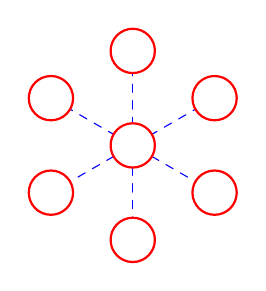
\begin{tikzpicture}[scale=0.8, font=\footnotesize, line join=round, line cap=round, >=stealth]
			\draw[dashed, blue] (90:1.5) -- (270:1.5);
			\draw[dashed, blue] (30:1.5) -- (210:1.5);
			\draw[dashed, blue] (150:1.5) -- (330:1.5);
			\foreach \angle in {90, 270, 30, 210, 150, 330} {
				\filldraw[fill=white, draw=red, thick] (\angle:1.5) circle (10pt);
			}
			\filldraw[fill=white, draw=red, thick] (0,0) circle (10pt);
		\end{tikzpicture}
	}
	\shortans[]{384}
	\loigiai{
		Để cứ ba ô hình tròn thẳng hàng đều chứa số $1$, số $1$ bắt buộc phải được xếp vào ô hình tròn ở vị trí trung tâm. Có $1$ cách xếp số $1$.\\
		Khi đó, tổng của ba ô hình tròn thẳng hàng bằng nhau khi và chỉ khi tổng của hai ô hình tròn ở hai đầu của mỗi đường thẳng là bằng nhau.\\
		Gọi ba cặp số ở hai đầu của ba đường thẳng là $(a;b)$, $(c;d)$ và $(e;f)$.\\
		Ta cần chọn ra $3$ cặp số phân biệt từ tập $X \setminus \{1\} = \{2; 3; 4; 5; 6; 7; 8; 9\}$ sao cho $a+b = c+d = e+f$.\\
		Ta có các trường hợp tổng bằng nhau như sau:
		\begin{itemize}
			\item Tổng bằng $9$, có $3$ cặp là $\{2;7\}$, $\{3;6\}$, $\{4;5\}$. Số cách chọn $3$ cặp là $\mathrm{C}_3^3 = 1$ cách.
			\item Tổng bằng $10$, có $3$ cặp là $\{2;8\}$, $\{3;7\}$, $\{4;6\}$. Số cách chọn $3$ cặp là $\mathrm{C}_3^3 = 1$ cách.
			\item Tổng bằng $11$, có $4$ cặp là $\{2;9\}$, $\{3;8\}$, $\{4;7\}$, $\{5;6\}$. Số cách chọn $3$ cặp là $\mathrm{C}_4^3 = 4$ cách.
			\item Tổng bằng $12$, có $3$ cặp là $\{3;9\}$, $\{4;8\}$, $\{5;7\}$. Số cách chọn $3$ cặp là $\mathrm{C}_3^3 = 1$ cách.
			\item Tổng bằng $13$, có $3$ cặp là $\{4;9\}$, $\{5;8\}$, $\{6;7\}$. Số cách chọn $3$ cặp là $\mathrm{C}_3^3 = 1$ cách.
		\end{itemize}
		Số cách chọn được $3$ bộ cặp số thỏa mãn điều kiện trên là $1+1+4+1+1 = 8$ (cách).\\
		Với mỗi bộ $3$ cặp số được chọn, ta tiến hành xếp chúng vào $6$ ô hình tròn còn lại (có hoán vị vị trí cho $3$ đường thẳng và hoán vị $2$ số trong mỗi cặp), khi đó số cách xếp là
		\[3! \cdot 2! \cdot 2! \cdot 2! = 48 \text{ (cách).}\]
		Vậy có tất cả $1 \cdot 8 \cdot 48 = 384$ cách xếp thỏa mãn bài toán.
	}
\end{ex}
%%%=============================%%%

